\section{系统实现}\label{chap:implementation}

本章分别介绍服务端、Android 客户端和 Web 客户端的具体实现过程，以及关键功能的实现细节。

\subsection{服务端实现}

\subsubsection{FastAPI 应用结构}

服务端基于 FastAPI 框架构建，采用模块化的项目结构。主要目录组织如下：

\begin{lstlisting}[language={}]
server/
+-- main.py                   # 应用入口、生命周期管理
+-- config.py                 # 配置项（JWT、数据库、队列等）
+-- database.py               # SQLite 数据库初始化与连接
+-- dependencies.py           # FastAPI 依赖注入（认证）
+-- api/v1/
|   +-- auth.py               # 认证路由（注册/登录/登出）
|   +-- invite.py             # 邀请码路由
|   +-- stego.py              # 隐写路由（双算法统一入口）
|   `-- ws.py                 # WebSocket 路由
+-- services/
|   +-- auth_service.py       # 密码哈希、JWT、用户 CRUD
|   +-- pulsar_service.py     # Pulsar 算法服务封装
|   +-- sparsample_service.py # SparSamp 算法服务封装
|   +-- ws_manager.py         # WebSocket 连接管理
|   `-- queue_service.py      # 离线消息队列
+-- services/sparsample/      # SparSamp 算法核心实现
|   +-- core.py               # 嵌入/提取/扩散采样/高斯量化
|   `-- guided_diffusion/     # UNet 模型定义
+-- sage/                     # SageMath 纠错码实现
`-- models/                   # 数据模型
\end{lstlisting}

应用启动时通过 FastAPI 的生命周期管理（lifespan）完成数据库初始化和定时任务注册。路由通过 \texttt{include\_router} 方法注册到主应用实例。CORS 中间件允许跨域请求以支持 Web 客户端访问。

\subsubsection{双算法隐写服务集成}

系统通过算法注册表模式实现 Pulsar 和 SparSamp 的统一管理。注册表结构维护每个算法的 ID、显示名称、模型列表和服务类引用。聊天模式的默认算法为 SparSamp（\texttt{CHAT\_DEFAULT\_ALGORITHM = "sparsample"}）。

\textbf{PulsarService} 采用类方法设计，主要包含：

\begin{itemize}
    \item \textbf{实例管理}：使用字典缓存 Pulsar 实例，以 \texttt{"模型ID:密钥十六进制"} 组合作为缓存键。首次请求时自动加载预训练模型并执行区域估计。
    \item \textbf{嵌入操作}：接收消息字节、模型ID和密钥，调用 Pulsar 的 \texttt{generate\_with\_regions} 方法生成含密图像，将图像保存为 PNG 格式并返回字节数据。
    \item \textbf{提取操作}：接收含密图像字节、模型ID和密钥，调用 \texttt{reveal\_with\_regions} 方法提取隐藏消息。
\end{itemize}

\textbf{SparSampService} 同样采用类方法设计，但内部实现更为复杂：

\begin{itemize}
    \item \textbf{状态缓存}：对每个（模型ID、密钥）对，首次请求时执行完整的 IDDPM 扩散采样流程，缓存中间状态（$x_1$、$\mu$、$\sigma$、最大容量）。后续请求直接使用缓存，实现瞬时返回。
    \item \textbf{嵌入操作}：将消息打包为比特序列，通过消息驱动采样机制逐像素嵌入——将消息段与伪随机数模加结合生成 MRN，使用 MRN 从量化分布中采样 bin 索引，并通过稀疏采样机制消除解码歧义，最终生成 $256 \times 256$ 的 PNG 图像。
    \item \textbf{提取操作}：使用相同的密钥和种子恢复扩散状态，从像素值反向推导 bin 索引，利用相同的 MRN 更新逻辑逐步缩小候选消息集合，直到唯一确定消息段。
\end{itemize}

两种算法均使用 \texttt{run\_in\_threadpool} 在线程池中执行 CPU 密集型操作，避免阻塞异步事件循环。

\subsubsection{WebSocket 连接管理}

\texttt{ConnectionManager} 类负责管理所有活跃的 WebSocket 连接，使用字典维护用户ID到 WebSocket 实例的映射关系。核心实现包括：

\begin{itemize}
    \item \textbf{连接建立}：验证 JWT 令牌后建立连接。若该用户已有活跃连接（多设备登录），先向旧连接发送 \texttt{kicked} 消息，并设置 5 秒延迟强制关闭。
    \item \textbf{消息路由}：根据消息中的目标用户ID查找对应的 WebSocket 连接，若目标用户在线则直接转发，否则将消息加入离线队列。
    \item \textbf{消息生命周期}：服务端为每条 chat 消息生成唯一 ID 和时间戳，向发送者返回 \texttt{ack} 确认，支持 \texttt{delivered}、\texttt{read} 和 \texttt{revoke} 状态的转发。
    \item \textbf{离线消息投递}：用户连接建立后，自动查询并投递该用户的所有缓存消息。
\end{itemize}

\subsubsection{离线消息队列}

离线消息使用 SQLite 的 \texttt{message\_queue} 表实现持久化存储。消息入队时设置 24 小时过期时间，服务端通过 \texttt{asyncio.create\_task} 启动定时清理任务，每 5 分钟删除过期消息。用户重新上线时，系统自动投递所有未过期消息并从队列中移除。

\subsection{Android 客户端实现}

\subsubsection{界面实现}

Android 客户端使用 Jetpack Compose 构建声明式 UI，采用 Material 3 Expressive 设计语言，主色调为薄荷色（\#4ECDC4），使用 Inter 字体族。主要包含以下页面：

\begin{itemize}
    \item \textbf{AuthScreen}：登录和注册界面，通过 \texttt{PrimaryTabRow} 实现标签切换。品牌标识为 EnhancedEncryption 图标 + "StegoCrypt" 文字。支持表单验证（用户名 3 字符以上，密码 6 字符以上）。
    \item \textbf{ChatListScreen}：会话列表，显示所有已接受的联系人，按最后消息时间排序。每行显示头像、显示名称、最后消息预览（文本或"隐写图像"图标）和时间戳。
    \item \textbf{ChatScreen}：聊天界面，顶部显示 E2EE 状态横幅（三种状态：自身未配置/对方未配置/已加密），中间为消息列表，底部为输入栏。支持普通消息和隐写消息的发送与接收。
    \item \textbf{ContactsScreen}：联系人列表，顶部显示好友请求入口（带未读计数），每行显示头像、名称和加密状态标签。
    \item \textbf{AddContactScreen}：通过邀请码添加联系人，支持搜索预览和备注输入。
    \item \textbf{ContactDetailScreen}：联系人详情页，支持配置对方的 E2EE 助记词、查看指纹、发起聊天和删除联系人。
    \item \textbf{RequestsScreen}：好友请求列表，支持接受、忽略和屏蔽三种操作。接受时自动处理队列中的暂存消息。
    \item \textbf{ProfileScreen}：个人设置页，包含邀请码管理（查看/复制/重置）和自身 E2EE 助记词配置（输入/保存/重置/指纹显示）。
    \item \textbf{StegoToolScreen}：独立隐写工具，通过 \texttt{SingleChoiceSegmentedButtonRow} 切换嵌入和提取两种模式，支持算法和模型选择。
\end{itemize}

页面导航使用 Jetpack Navigation Compose 实现，底部导航栏提供消息、联系人、隐写工具和我的四个入口。

\subsubsection{Room 数据库实现}

使用 Room 持久化库定义本地数据库（版本 2），包含以下 DAO 操作：

\begin{itemize}
    \item \textbf{ContactDao}：联系人的增删改查，支持按用户ID查询和全量查询，支持更新 E2EE 对方密钥字段。
    \item \textbf{MessageDao}：聊天消息的插入、按联系人ID查询（按时间排序）和状态更新。
    \item \textbf{BlacklistDao}：黑名单的增删查。
    \item \textbf{UserSettingsDao}：当前用户 E2EE 配置的读写（单行表，ID 固定为 0），支持 Flow 观察。
\end{itemize}

数据库版本 1 到版本 2 的迁移添加了联系人表的 E2EE 字段（\texttt{peerPhrase}、\texttt{peerUserKeyHex}、\texttt{peerFingerprintHex}）和 \texttt{user\_settings} 表。

\subsubsection{端到端加密实现}

本节介绍\cref{chap:design}章中端到端加密设计的具体代码实现。\texttt{CryptoUtils.kt} 封装了所有密码学操作，包含以下常量和方法：

\begin{itemize}
    \item \textbf{常量}：\texttt{SEED\_SALT}（"stegochat-seed-v1"）、\texttt{MKEY\_SALT}（"stegochat-mkey-v1"）、\texttt{MKEY\_INFO}（"e2ee"）、\texttt{PBKDF2\_ITER}（100,000）。
    \item \textbf{deriveUserKey(phrase)}：使用 PBKDF2WithHmacSHA256 从助记词派生 256 位用户密钥。
    \item \textbf{deriveMkey(selfKey, peerKey)}：按字典序排列两个用户密钥，拼接后使用 HKDF（HMAC-SHA-256）派生 32 字节消息密钥。
    \item \textbf{fingerprint(userKey)}：计算用户密钥的 SHA-256，取前 8 字节作为指纹。
    \item \textbf{SealedMessage.seal(mkey, plaintext)}：生成 12 字节随机 nonce，执行 AES-256-GCM 加密，构造 JSON 信封 $\{v:1, n:..., c:...\}$，base64url 编码。
    \item \textbf{SealedMessage.tryOpen(mkey, sealed)}：base64url 解码、JSON 解析、AES-256-GCM 解密。失败返回 null。
\end{itemize}

消息密钥（mkey）在 \texttt{ChatViewModel} 中通过 \texttt{combine} 操作符自动重算：当活跃联系人 ID、用户自身 E2EE 配置或联系人列表发生变化时，自动为当前聊天对象派生新的 mkey。

\subsubsection{WebSocket 客户端实现}

\texttt{WsClient} 类使用 OkHttp 库实现 WebSocket 客户端：

\begin{itemize}
    \item URL 构造：将 HTTP(S) 地址替换为 WS(S) 地址，附加 \texttt{?token=<jwt>} 查询参数。
    \item 消息解析：接收到的 JSON 文本解析为 \texttt{WsMessage} 对象，通过 \texttt{SharedFlow} 分发给 ViewModel。
    \item 重连机制：指数退避策略，最大间隔 30 秒，最多重连 10 次。
    \item 踢出检测：WebSocket 关闭码 4001 或 HTTP 401/403 触发踢出流程。
\end{itemize}

\texttt{ChatViewModel} 在 \texttt{handleWsMessage} 方法中按消息类型分发处理：

\begin{itemize}
    \item \textbf{chat}：检查黑名单、判断是否为新联系人（好友请求场景）、执行 E2EE 解密、保存到本地数据库、发送 delivered 回执。
    \item \textbf{ack}：更新消息状态为 "sent"。
    \item \textbf{delivered}：更新消息状态为 "delivered"。
    \item \textbf{read}：更新消息状态为 "read"。
    \item \textbf{revoke}：标记消息为已撤回，清除内容。
    \item \textbf{kicked}：断开连接，发射踢出事件。
\end{itemize}

\subsubsection{隐写功能实现}

聊天界面中的隐写模式通过一个切换开关控制，启用条件为邀请码已加载且 E2EE 已配置：

\begin{enumerate}
    \item 用户切换到隐写模式后，界面显示容量指示器和 XOR 密钥信息。
    \item 发送时先调用 \texttt{SealedMessage.seal} 对明文加密，再将 SealedMessage 字符串作为载荷调用 \texttt{/api/v1/stego/embed} 接口。密钥由双方邀请码 XOR 生成。
    \item 嵌入成功后，将含密图像的 base64 数据作为 \texttt{stego} 类型消息通过 WebSocket 发送给对方。
    \item 接收方收到隐写消息后，在聊天界面显示图像预览。长按可选择"提取秘密消息"，调用 \texttt{/api/v1/stego/extract} 接口提取载荷，再调用 \texttt{SealedMessage.tryOpen} 解密还原明文。
\end{enumerate}

独立隐写工具（StegoToolScreen）不涉及 E2EE，用户手动输入消息和密钥，支持选择算法和模型。

\subsection{Web 客户端实现}

\subsubsection{Vue 组件结构}

Web 客户端的主要页面组件如\cref{tab:web_views}所示。

\begin{table}[htb!]
    \caption{Web 客户端页面组件}
    \centering
    \begin{tabular}{llp{5cm}}
        \hline
        \textbf{组件} & \textbf{路由} & \textbf{功能} \\
        \hline
        AuthView & /login, /register & 登录注册（标签切换） \\
        ChatListView & /chats & 会话列表 \\
        ChatView & /chat/:id & 单个聊天（含 E2EE 状态） \\
        ContactsView & /contacts & 联系人列表 \\
        AddContactView & /contacts/add & 添加联系人 \\
        ContactDetailView & /contacts/:id & 联系人详情（E2EE 配置） \\
        RequestsView & /contacts/requests & 好友请求列表 \\
        ProfileView & /profile & 个人设置（邀请码 + E2EE） \\
        EmbedView & /embed & 独立隐写嵌入工具 \\
        ExtractView & /extract & 独立隐写提取工具 \\
        \hline
    \end{tabular}
    \label{tab:web_views}
\end{table}

公共组件包括：\texttt{SideNav}（侧边导航栏，64px 宽，4 个导航入口）、\texttt{MessageBubble}（消息气泡，支持文本和隐写图像，右键菜单提供提取和保存操作）、\texttt{MessageInput}（输入栏，支持隐写模式切换和容量指示）。

\subsubsection{Pinia 状态管理}

使用 Pinia 管理全局状态，定义了四个 Store：

\begin{itemize}
    \item \textbf{AuthStore}：管理用户认证状态。令牌和用户信息持久化到 \texttt{localStorage}。\texttt{verify} 方法在应用启动时验证令牌有效性。\texttt{logout} 清除所有本地数据，\texttt{onKicked} 仅清除令牌。
    \item \textbf{ChatStore}：管理 WebSocket 连接和消息收发。维护消息密钥（mkey，内存驻留）、邀请码、活跃联系人等状态。实现了完整的消息生命周期处理（ack/delivered/read/revoke）。隐写密钥通过双方邀请码 XOR 计算。
    \item \textbf{ContactStore}：管理联系人列表和黑名单。支持通过邀请码添加联系人、配置对方 E2EE 助记词、屏蔽和取消屏蔽用户。
    \item \textbf{SettingsStore}：管理当前用户的 E2EE 配置（助记词、用户密钥、指纹），持久化到 IndexedDB 的 \texttt{settings} 存储。应用启动时通过 \texttt{hydrate} 方法恢复状态。
\end{itemize}

\subsubsection{IndexedDB 本地存储}

使用 idb 库封装 IndexedDB 操作，数据库名 \texttt{stego-app}，版本 2，包含四个对象存储：

\begin{itemize}
    \item \textbf{contacts}：联系人记录，主键 \texttt{user\_id}，包含 E2EE 对方密钥字段。
    \item \textbf{messages}：聊天消息，主键 \texttt{id}，按 \texttt{contact\_id} 和 \texttt{created\_at} 建立索引。
    \item \textbf{blacklist}：黑名单，主键 \texttt{user\_id}。
    \item \textbf{settings}：应用设置，主键 \texttt{key}，存储 E2EE 自身配置。
\end{itemize}

\subsubsection{端到端加密实现}

Web 端的 E2EE 实现位于 \texttt{src/crypto/e2ee.ts}，使用 Web Crypto API 实现所有密码学操作。关键常量（\texttt{SEED\_SALT}、\texttt{MKEY\_SALT}、\texttt{MKEY\_INFO}、\texttt{PBKDF2\_ITER}）与 Android 端和 Python 服务端保持一致。

密钥派生流程与 Android 端完全对称：\texttt{deriveUserKey} 使用 \texttt{crypto.subtle.deriveBits} 实现 PBKDF2，\texttt{deriveMkey} 使用 \texttt{crypto.subtle.deriveBits} 实现 HKDF。SealedMessage 的 JSON 信封格式和 base64url 编码规则与 Android 端完全一致，确保跨平台消息互通。

base64url 编码采用 URL 安全变体（\texttt{-} 替代 \texttt{+}，\texttt{\_} 替代 \texttt{/}），去除填充符 \texttt{=}，与 Android 端的 \texttt{java.util.Base64.getUrlEncoder().withoutPadding()} 对齐。

\subsubsection{WebSocket 与隐写功能}

Web 客户端的 WebSocket 实现使用浏览器原生 \texttt{WebSocket} API，封装为 \texttt{WsClient} 单例类。连接 URL 从 API 基础地址推导（HTTP 替换为 WS），支持指数退避重连（最大间隔 30 秒，最多 10 次）。

隐写消息收发流程与 Android 端一致：发送时先加密（\texttt{sealMessage}）再嵌入（\texttt{stegoApi.embed}），接收时先提取（\texttt{stegoApi.extract}）再解密（\texttt{openStegoPayload}）。隐写图像在 Web 端以纯 base64 字符串存储（不含 \texttt{data:} 前缀），渲染时动态添加前缀。

\subsection{关键功能实现细节}

\subsubsection{单端登录机制}

单端登录涉及服务端和客户端的协同处理：

\begin{enumerate}
    \item \textbf{服务端}：\texttt{ConnectionManager.connect} 方法在新连接到来时，检查该用户是否已有活跃连接。若有，先发送 \texttt{kicked} 消息，然后创建异步任务在 5 秒后强制关闭旧连接（关闭码 4001）。
    \item \textbf{Android 客户端}：\texttt{WsClient} 监听关闭码 4001，通过 \texttt{SharedFlow} 发射踢出事件。\texttt{ChatViewModel} 收到后断开 WebSocket，通知 UI 层显示提示并跳转登录页。
    \item \textbf{Web 客户端}：\texttt{WsClient} 监听关闭码 4001，触发 \texttt{kicked} 事件。ChatStore 断开连接后通过 DOM 自定义事件通知 \texttt{App.vue} 执行页面跳转。
\end{enumerate}

主动登出清除所有本地数据（令牌、聊天记录、联系人、E2EE 配置），而被踢出仅清除令牌，保留聊天记录和 E2EE 配置。单端登录的时序交互如\cref{fig:single_device}所示。

\begin{figure}[htb!]
    \centering
    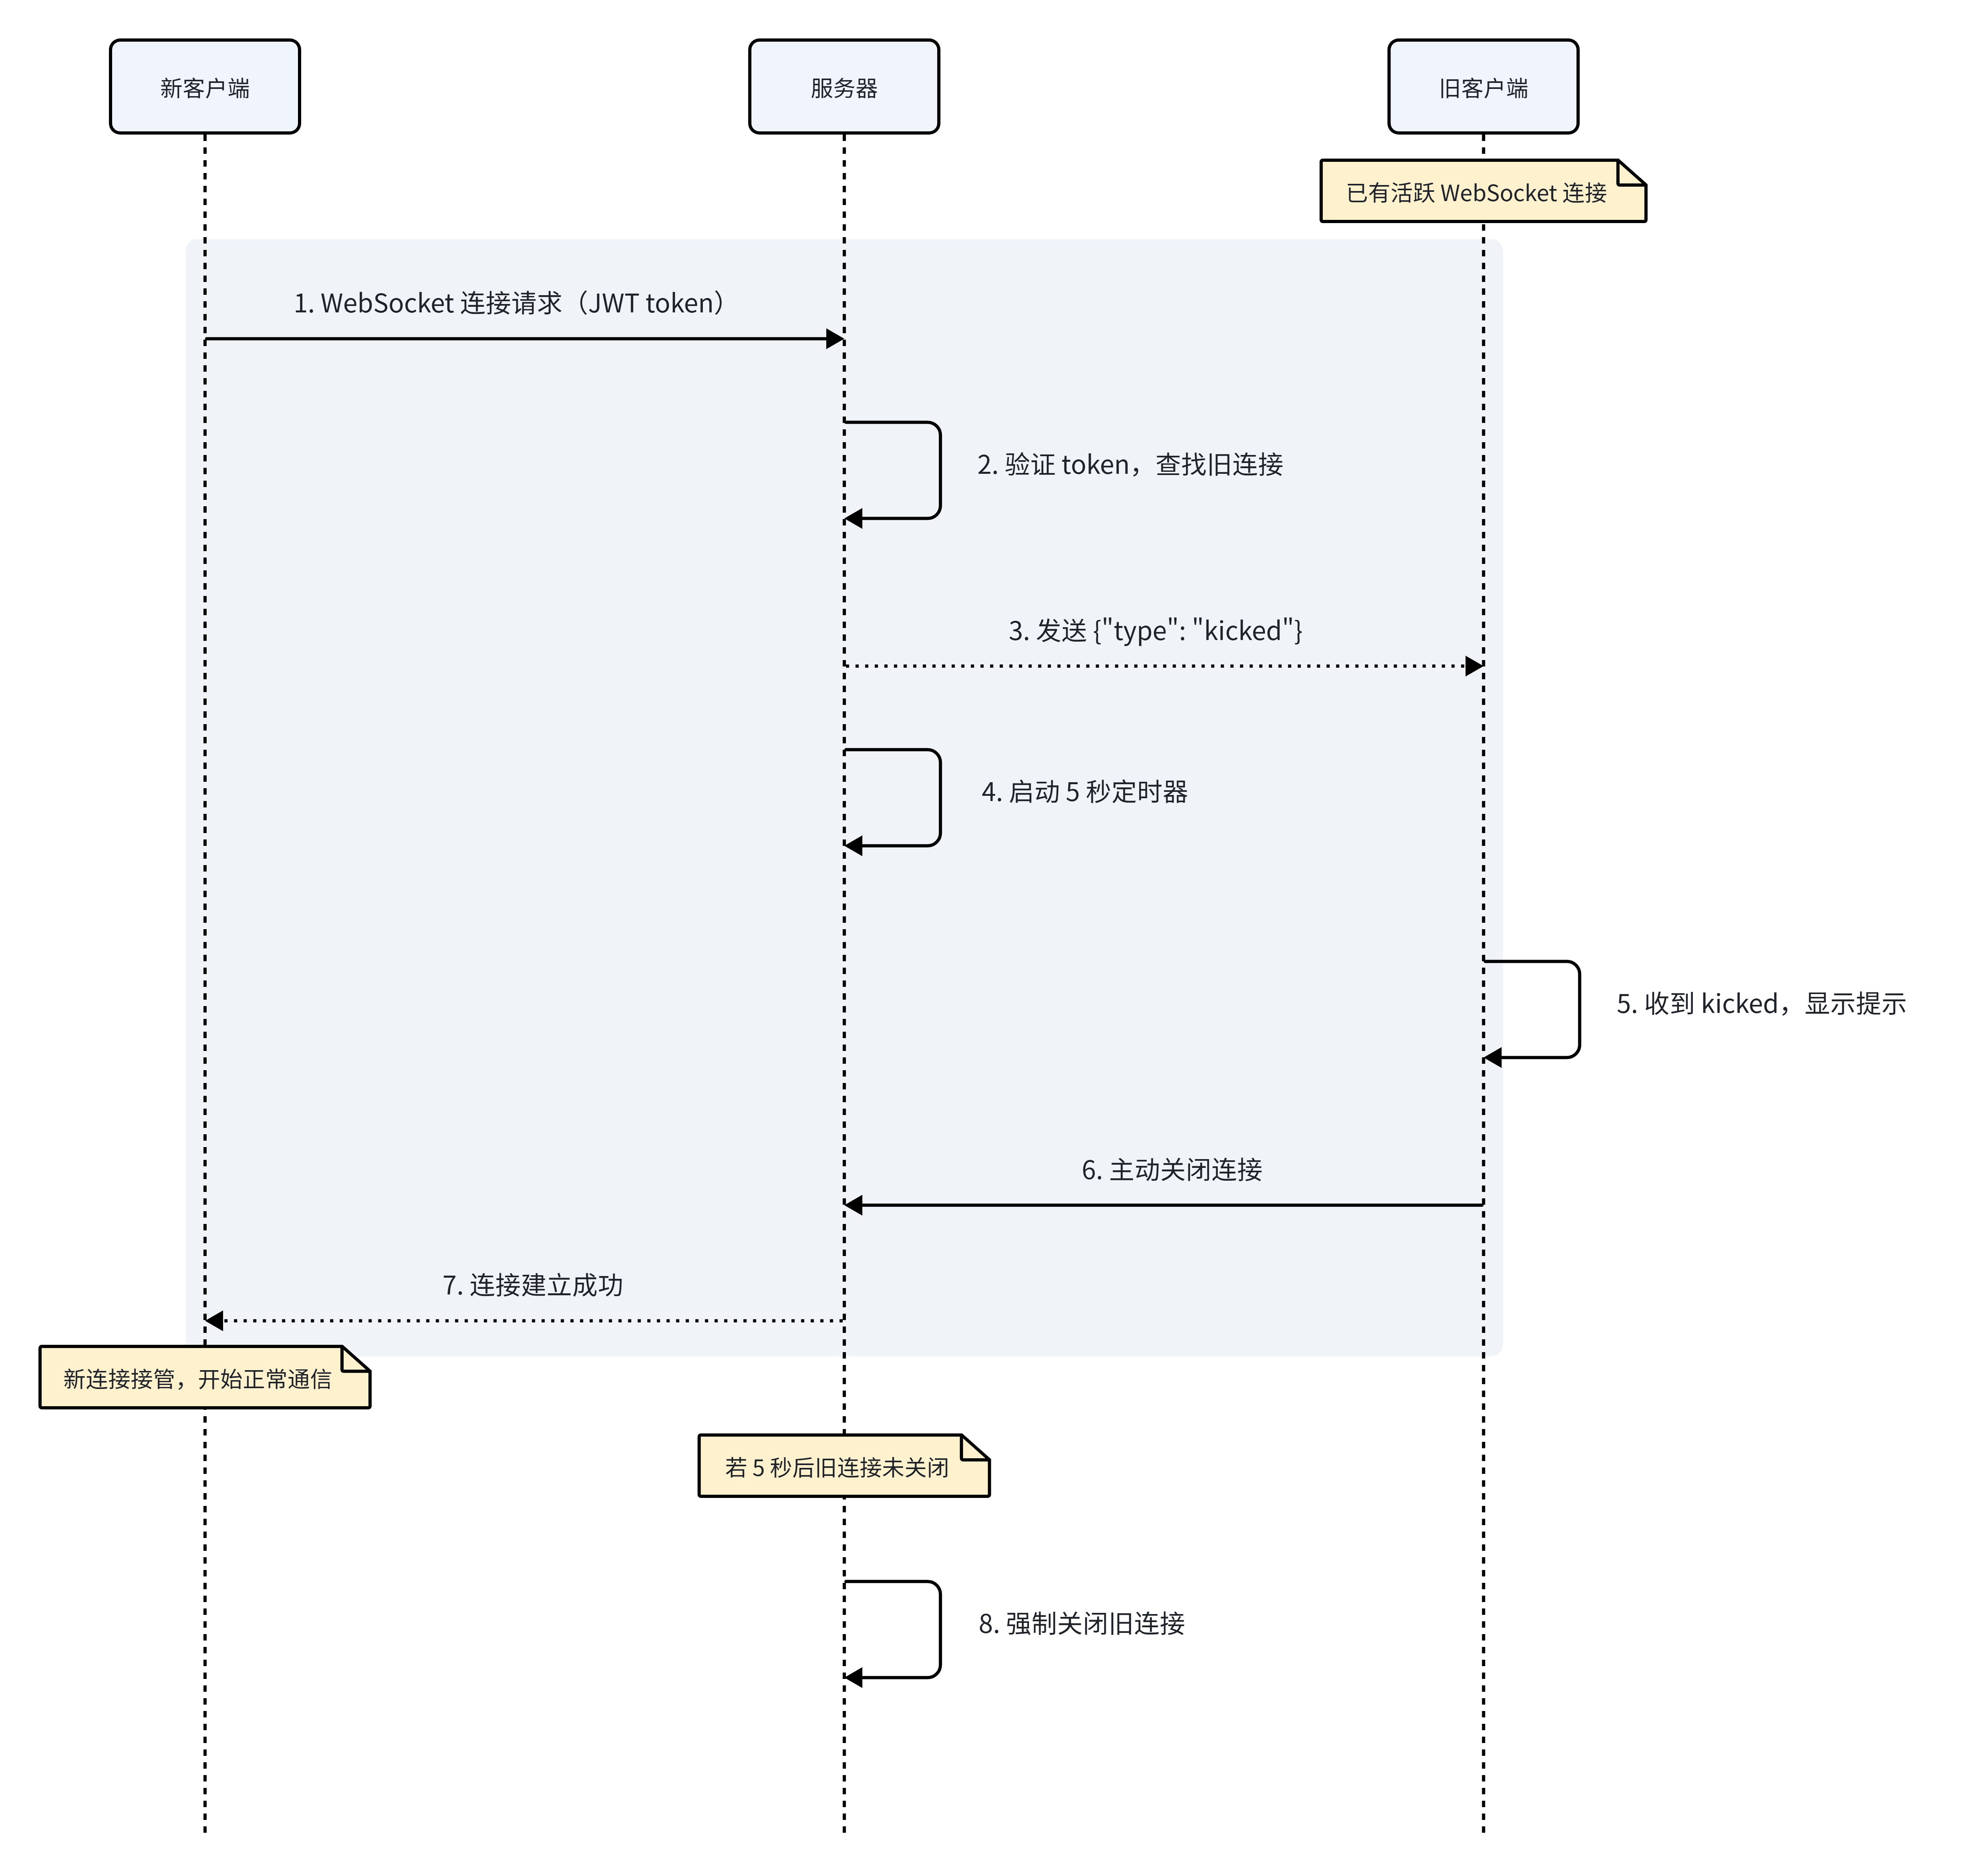
\includegraphics[width=0.85\textwidth]{img/ch4_single_device.png}
    \caption{单端登录时序}
    \label{fig:single_device}
\end{figure}

\subsubsection{好友请求流程}

好友添加采用基于邀请码的异步请求机制：

\begin{enumerate}
    \item 用户 A 输入用户 B 的邀请码，客户端调用 \texttt{/api/v1/invite/\{code\}} 查询对应用户信息。
    \item 确认后，客户端在本地数据库添加联系人（状态为 "accepted"），并通过 WebSocket 向用户 B 发送 \texttt{first\_contact} 类型的 chat 消息。
    \item 用户 B 收到消息时，若发送者不在联系人列表中，自动创建待处理请求。用户 B 可选择接受、忽略或屏蔽。
    \item 接受时，联系人添加到本地数据库，队列中的暂存消息被处理。
\end{enumerate}

需要处理的边界情况包括：重复请求的去重（通过检查联系人是否已存在）、离线请求的暂存与恢复、接受请求时恢复所有暂存的聊天消息等。好友请求流程如\cref{fig:friend_request}所示。

\begin{figure}[htb!]
    \centering
    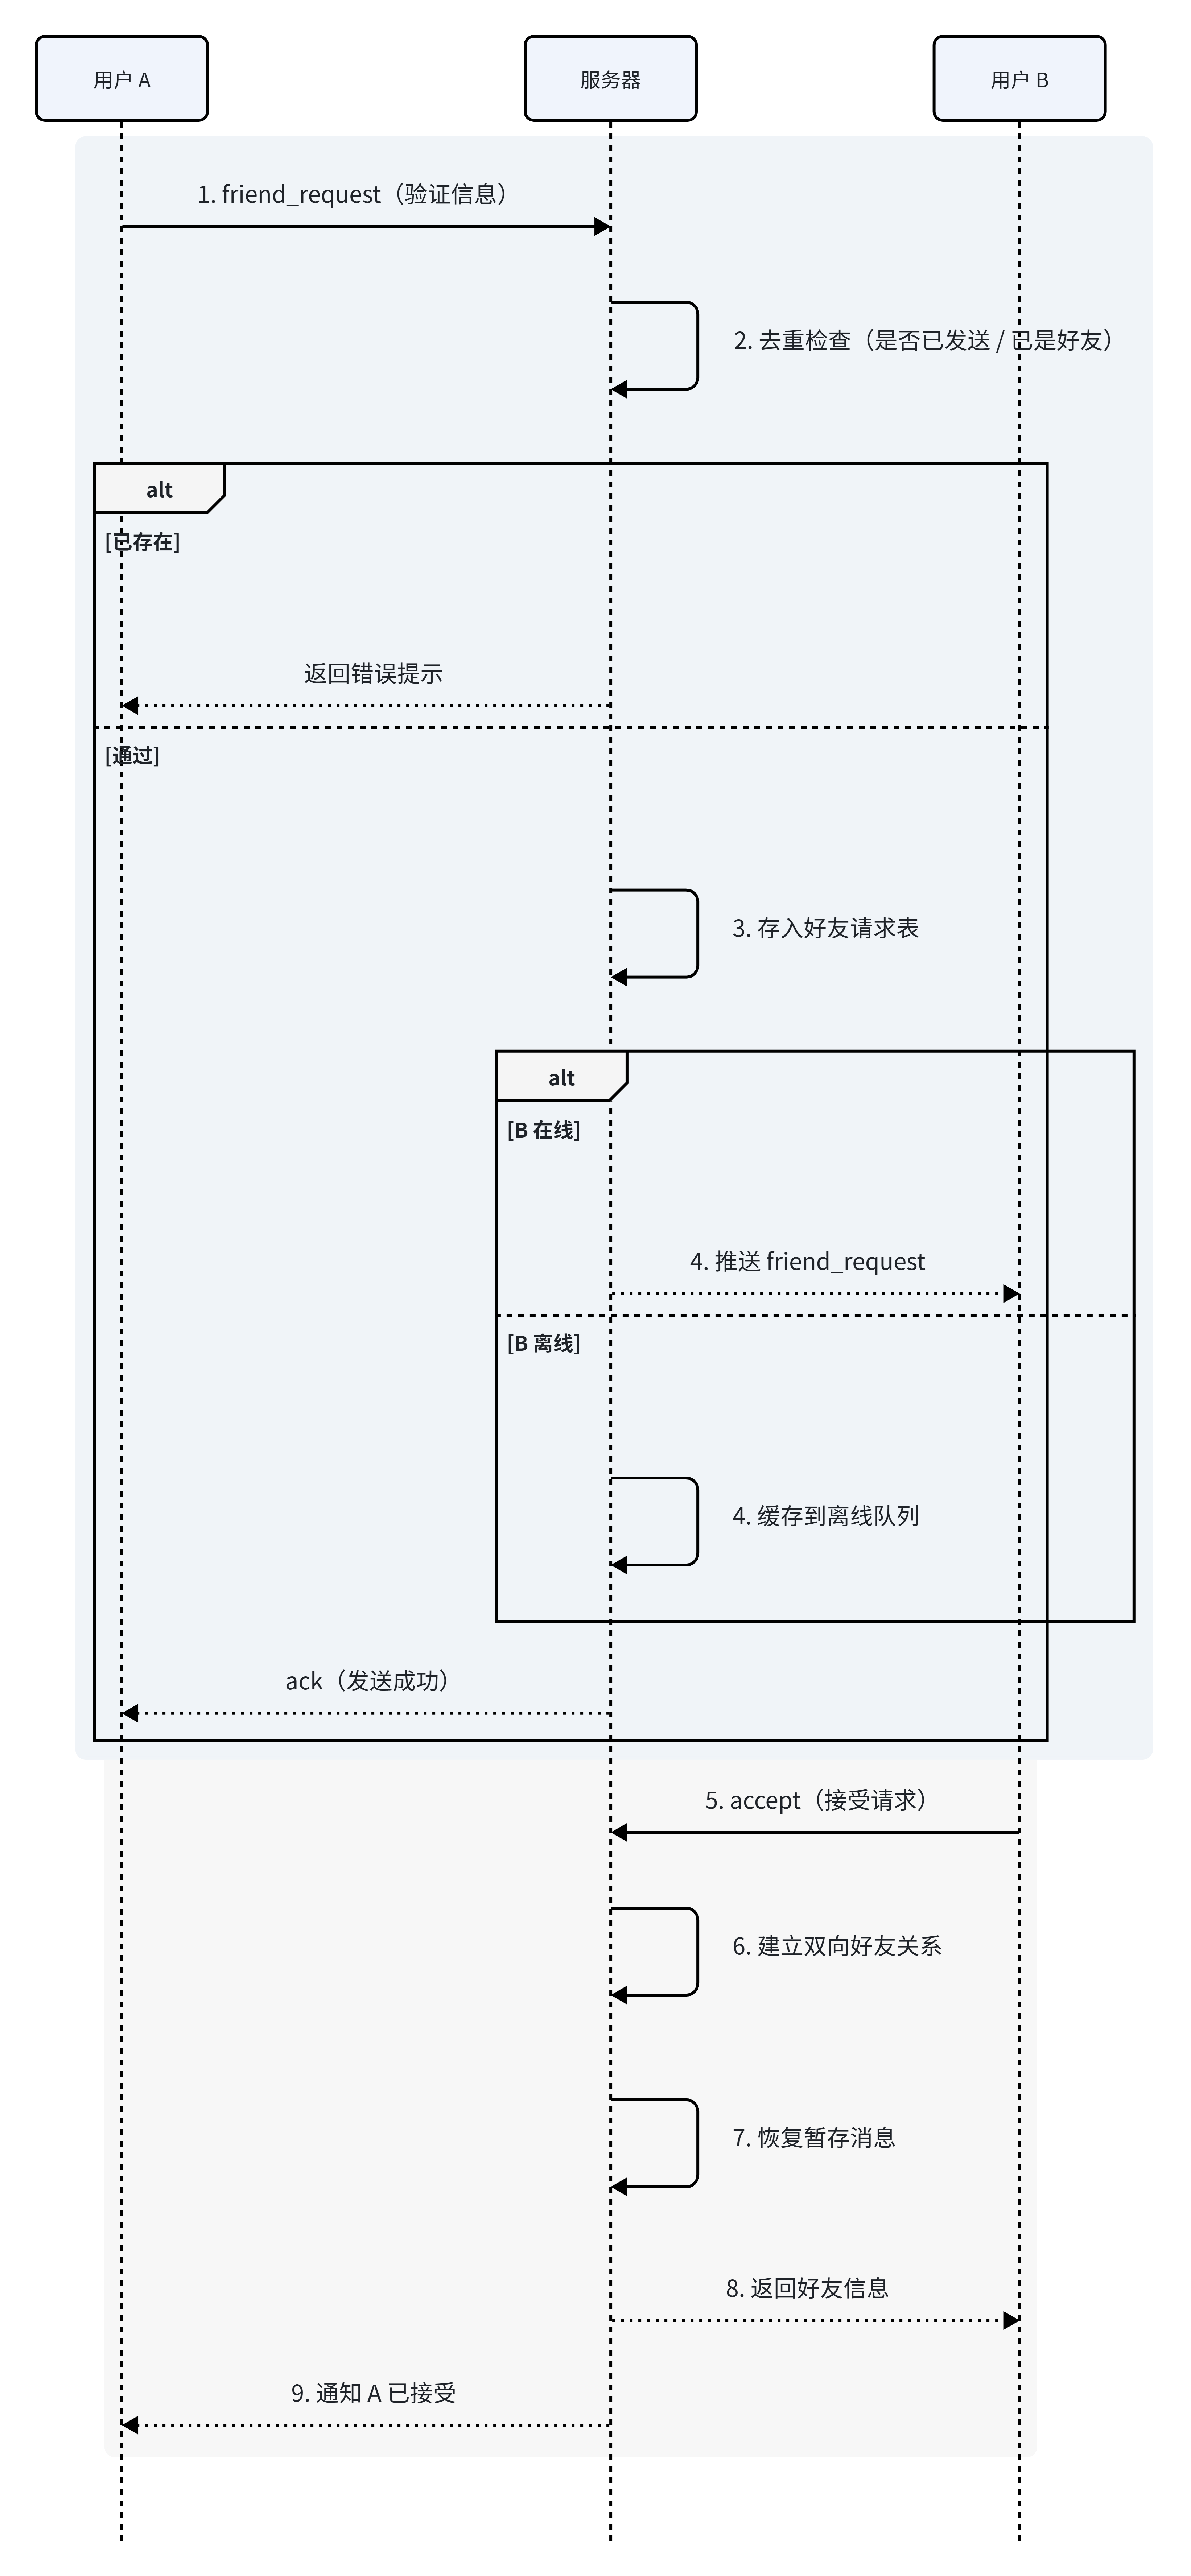
\includegraphics[width=0.85\textwidth]{img/ch4_friend_request.png}
    \caption{好友请求流程}
    \label{fig:friend_request}
\end{figure}

\subsubsection{隐写消息收发流程}

隐写消息的完整收发流程如下：

\begin{enumerate}
    \item \textbf{发送方}：用户切换到隐写模式，输入文本消息。客户端获取双方邀请码，XOR 计算隐写密钥。先调用 \texttt{SealedMessage.seal} 加密明文，再将密封字符串作为载荷调用嵌入 API。API 返回含密图像的 base64 数据后，通过 WebSocket 以 \texttt{stego} 类型发送。
    \item \textbf{服务端}：接收 WebSocket 消息，根据目标用户ID转发（或入离线队列）。服务端不解析 \texttt{stego\_image} 的内容。
    \item \textbf{接收方}：收到 \texttt{stego} 消息后，在聊天界面显示图像预览。用户选择提取，客户端使用相同的隐写密钥调用提取 API，得到密封字符串后调用 \texttt{SealedMessage.tryOpen} 解密还原明文。
\end{enumerate}

隐写消息的完整收发时序如\cref{fig:stego_message}所示。

\begin{figure}[htb!]
    \centering
    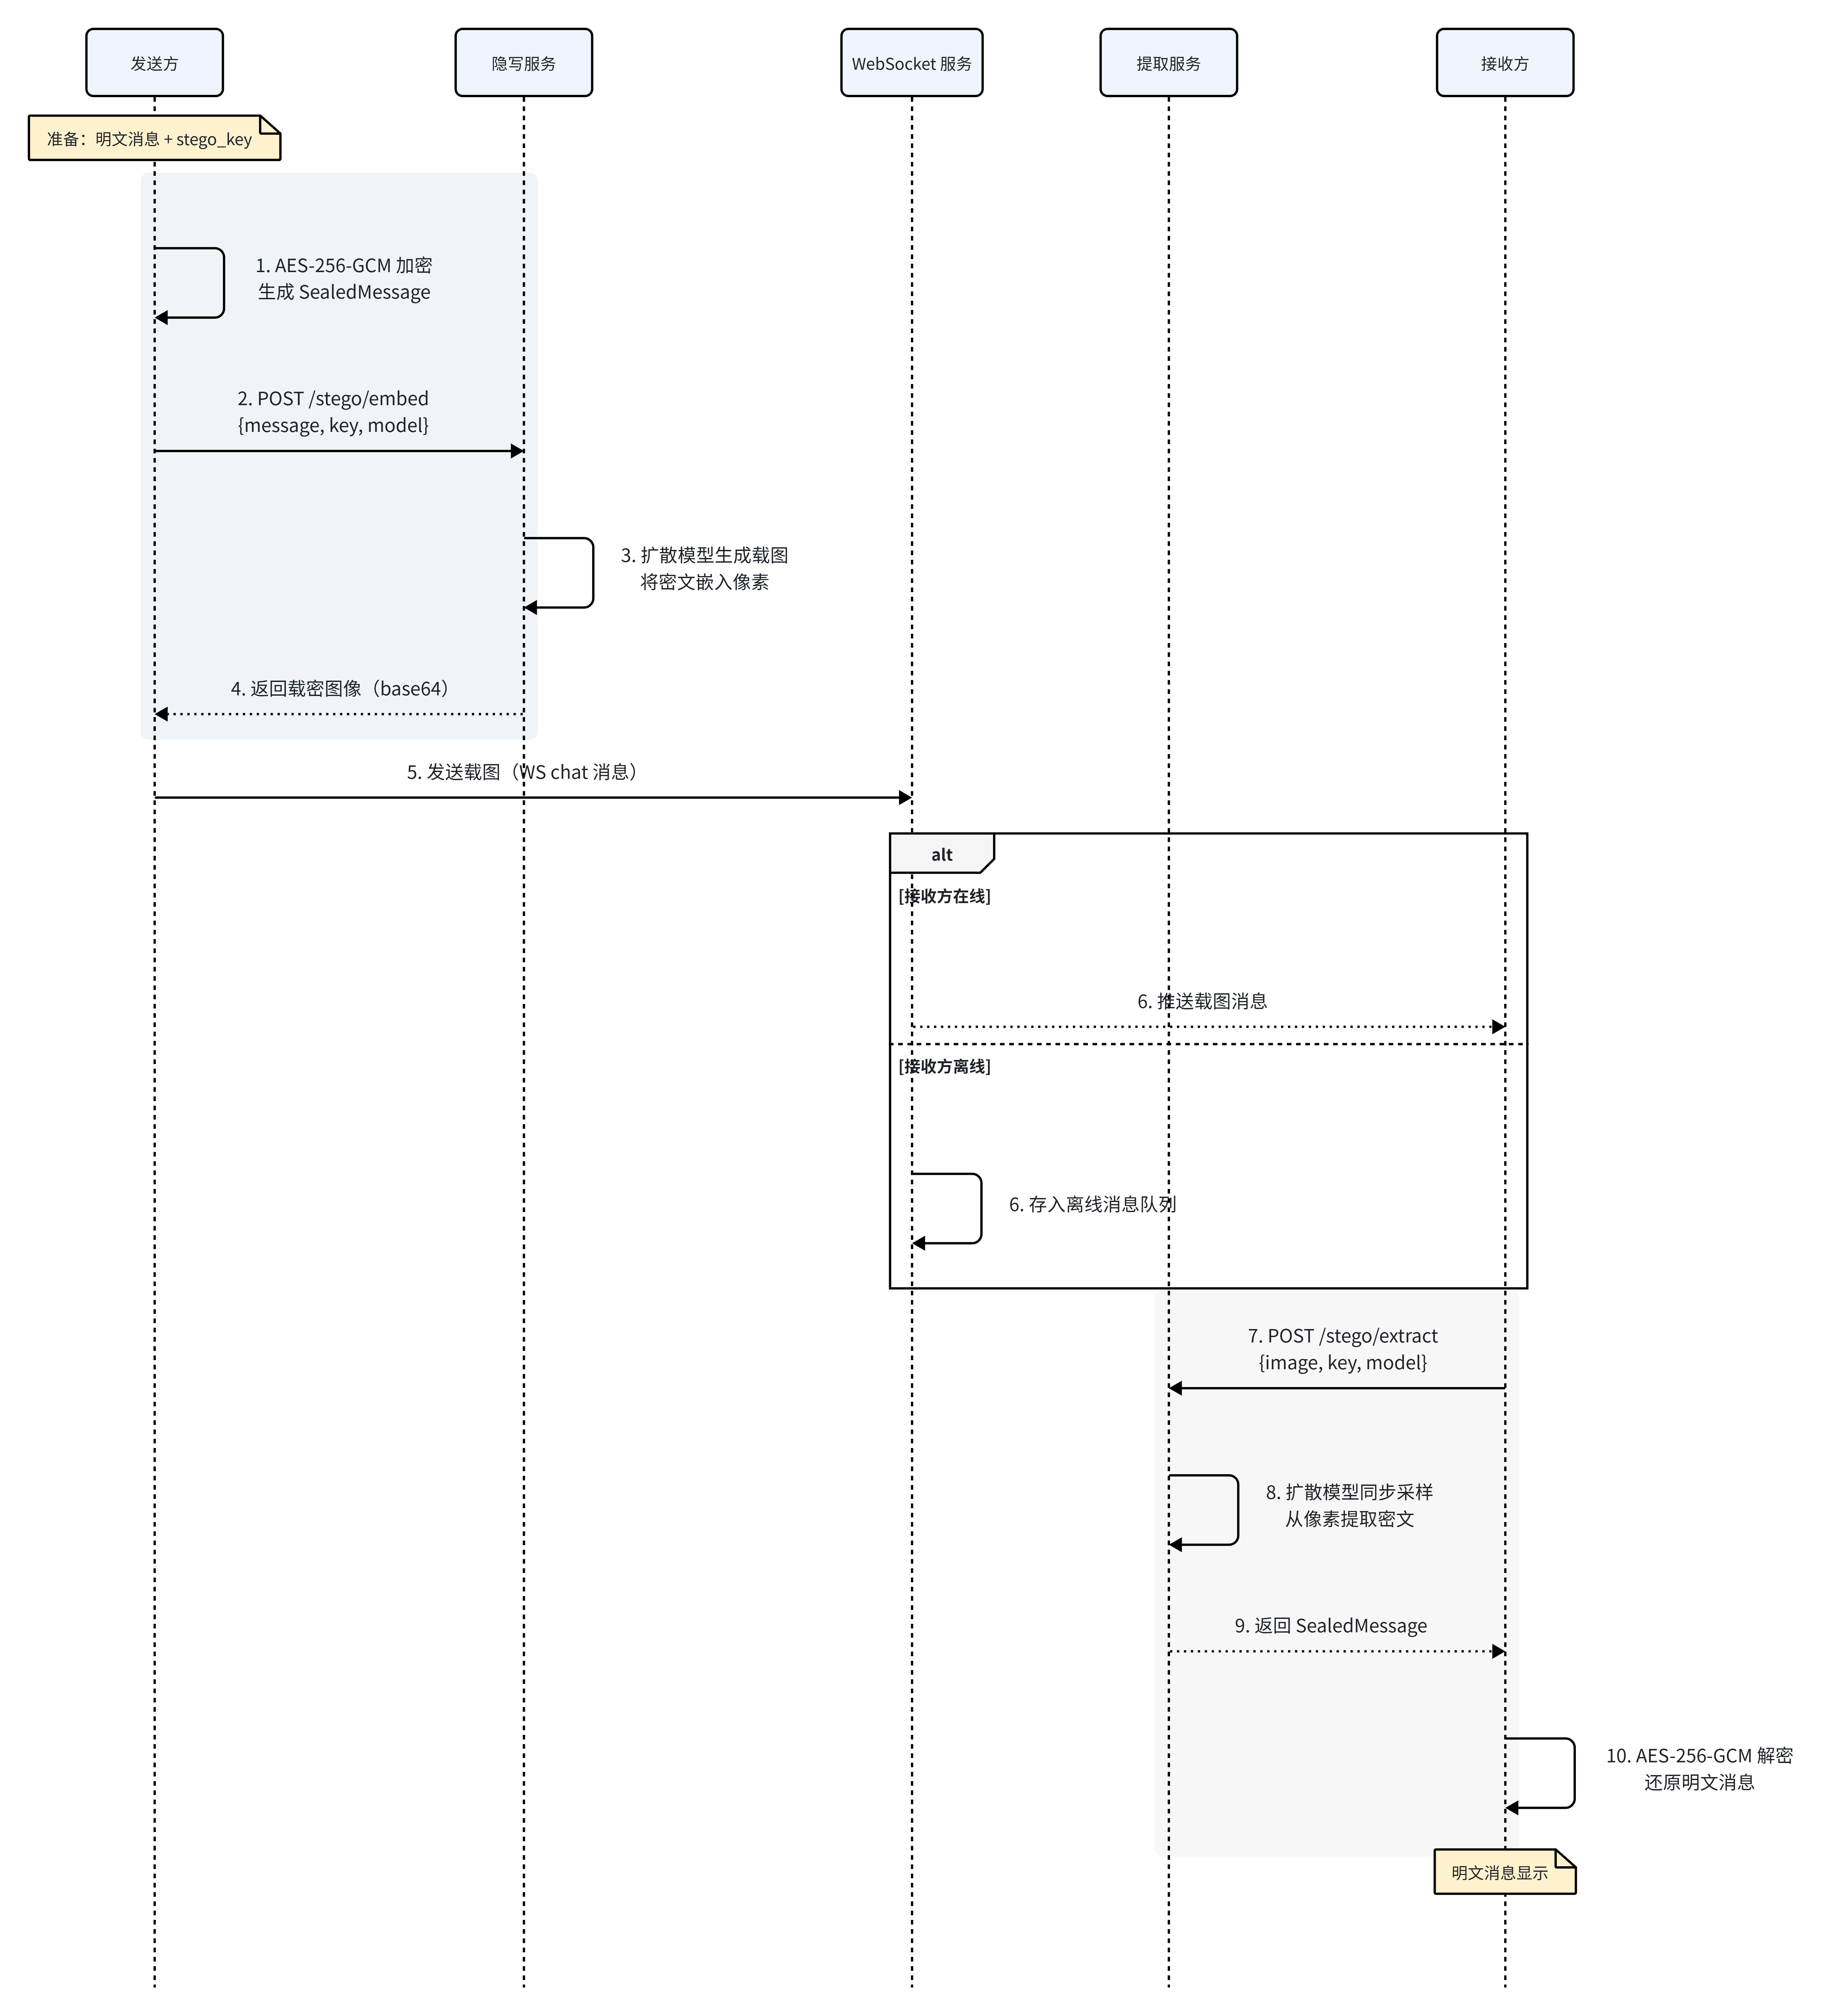
\includegraphics[width=0.85\textwidth]{img/ch4_stego_message.png}
    \caption{隐写消息收发时序}
    \label{fig:stego_message}
\end{figure}

\subsection{本章小结}

本章详细介绍了系统三个组件的具体实现过程。服务端通过模块化的 FastAPI 应用集成了双算法隐写引擎、WebSocket 通信（含完整消息生命周期）和离线消息队列；Android 客户端基于 MVVM 架构使用 Jetpack Compose 构建了包含 9 个页面的完整 UI 和数据管理层；Web 客户端使用 Vue.js 3、Pinia 和 Tailwind CSS 实现了与 Android 端功能对齐的浏览器应用。同时，本章重点阐述了端到端加密的跨平台实现、双算法隐写服务的统一接口设计、单端登录、好友请求和隐写消息收发等关键功能的实现细节。
